\documentclass{beamer}

\usepackage{amsmath}
\usepackage{graphicx}
\title{Probabilistic Analysis and Randomized Algorithms}
\author{Geoffrey Matthews}
\newcommand{\bi}{\begin{itemize}}
\newcommand{\ei}{\end{itemize}}
\newcommand{\bn}{\begin{enumerate}}
\newcommand{\en}{\end{enumerate}}
\newcommand{\set}[1]{\ensuremath{\left\{#1\right\}}}
\newcommand{\sect}[1]{
\section{#1}
\begin{frame}[fragile]\frametitle{#1}
}
\newcommand{\pr}[1]{\ensuremath{\mbox{Pr}\left\{#1\right\}}}


\begin{document}

\begin{frame}
\maketitle
\end{frame}

\sect{Goals}
\bi
\item Present difference between probabilistic analysis and randomized
  algorithms.
\item Present technique of indicator random variables.
\item Analysis of randomized algorithm.
  \ei
\end{frame}

\sect{The Hiring Problem}

\bi
\item
  You are using an employment agency to hire a new office assistant.
\item
  The agency sends you one candidate each day.
\item
  You interview the candidate and must immediately decide whether or not to
hire that person and fire the current one.
\item
  Cost to interview is $c_i$ per candidate
Cost to hire is $c_h$ per candidate.
\item
  Assume that $c_h > c_i$.
\item
  You are committed to always have the best candidate seen so
  far. 
\item
  {\bf Goal:}
  Determine what the price of this strategy will be.
\ei

\end{frame}


\sect{Hire-Assistant}

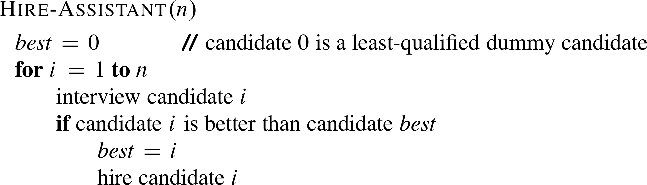
\includegraphics{Hire-Assistant.pdf}

\end{frame}

\sect{Costs}

If there are $n$ candidates and we hire $m$ of them, cost is
\[
O(nc_i + mc_h)
\]
\bi
\item Have to pay $nc_i$ no matter what.
\item Focus on $mc_h$.
\item $mc_h$ depends on the order of candidates.
\item This is a common scenario.
\ei

\end{frame}

\sect{Worst-case analysis}
\pause
\bi
\item Candidates are sorted worst to best.
\item We hire all candidates.
\item Cost is
  \[ O(nc_i + nc_h) = O(nc_h) \]
\ei
\end{frame}


\sect{Probabilistic analysis}
\bi
\item
  In general we have no control over the order.
\item
  We could assume candidates come in random order.
\item
  Assign a rank to reach candidate: $\mbox{rank}(i) \in
  \{1,2,...,n\}$.

  No ties.
\item
  The list $(\mbox{rank}(1),\mbox{rank}(2),...\mbox{rank}(n))$
  is a permutation of $(1,2,...,n)$.
\item
  The list of ranks is equally likely to be any one of the $n!$
  permutations.
\item
  The ranks form a {\bf uniform random permutation}.
  \ei

\end{frame}

\sect{Problem of probabilistic analysis}
\bi
\item We must use knowledge of the distribution of inputs,
  or make assumptions about it.
\item
  The expectation is over this distribution.
\item
  The technique requires that we can make reasonable assumptions about
  the input.
\item
  Also that we can successfully model the presumed input distribution.
  
\ei
\end{frame}

\sect{Randomized algorithms}

\bi
\item
  We might not know the input distribution, or be able to model it.
\item
  Instead, we randomize within the algorithm to impose a distribution.
  
\ei
\end{frame}

\sect{Randomized-Hire-Assistant}

Change the scenario:
\bi
\item The employment agency sends us a list of all candidates in
  advance.
\item
  On each day, we randomly choose a candidate from the list.
\item
  Instead of relying on the input distribution, we impose a uniform
  random one.
\ei

\end{frame}

\sect{What makes an algorithm randomized}


\bi
\item
  An algorithm is {\bf randomized}
  if its behavior is determined in part by values produced by a
  {\bf random-number generator}.
\item
  {\tt RANDOM(a,b)}
  returns an integer $r$, where $a \leq r \leq b$
  and each of the $b - a +1$
possible values of $r$ is equally likely.
\item
  In practice, {\tt RANDOM} is
  implemented by a {\bf pseudorandom-number generator},
  which is a deterministic method returning numbers that
  ``look'' random and pass
  statistical tests.
\ei
\end{frame}

\sect{Indicator random variables}
\bi
\item
A simple yet powerful technique for computing the expected value of a random
variable.
\item
Helpful in situations in which there may be dependence.
\item
  Given a sample space and an event $A$,
  we define the indicator random variable
  \[
  I\set{A} = \left\{\begin{array}{ll}
  1 & \mbox{ if $A$ occurs}\\
  0 & \mbox{ if $A$ does not occur}
  \end{array}\right.
  \]
\item
  {\bf Lemma}
  
For an event $A$, let $X_A = I\set{A}$. Then $E[X_A] = \pr{A}$.
\item
  {\bf Proof}

  Letting $\overline{A}$ be the complement of $A$, we have
  \begin{align*}
    E[X_A]
    &= E[I\set{A}]\\
    &= 1\cdot\pr{A} + 0\cdot\pr{\overline{A}}\\
    &= \pr{A}
  \end{align*}
  
\ei
\end{frame}

\sect{Simple example}

\bi
\item
  Determine expected number of heads if we flip a fair coin.
\item
  Sample space: \set{H,T}
\item
  $\pr{H} = \pr{T} = 1/2$
\item
  $X_H = I\set{H}$.
\item
  $X_H$ counts number of heads in one flip.
\item
  Since $\pr{H} = 1/2$, lemma says $E[X_H] = 1/2$.
  \ei


\end{frame}

\sect{More complicated example}
\bi
\item Expected number of heads in $n$ flips.
  Let $X$ be a random variable for number of heads in $n$ flips.
\item
  \[
  E[X] = \sum_{k=0}^n k \cdot \pr{X=k}
  \]
\item
  Instead, define $X_i = I\set{\mbox{the $i$th flip is $H$}}$, so
 $X = \sum_{i=1}^n X_i$
\item
  Lemma says $E[X_i] = \pr{H} = 1/2$.
  \begin{align*}
    E[X]
    &= E\left[\sum_{i=1}^n X_i\right] \\
    &=   \sum_{i=1}^n E[X_i] \\
    &=   \sum_{i=1}^n 1/2 = n/2
  \end{align*}
  
\ei
\end{frame}

\sect{The hiring problem analysis}
\bi
\item
  Assume canddiates arrive in random order.
\item
  Let $X$ be the RV that is the number of times we hire
  someone.
\item
  Define $X_i = I\set{\mbox{candidate $i$ is hired}}$
\item
  Candidate $i$ is hired iff $i$ is better than $1,2,...,i-1$.
\item
  $\pr{\mbox{candidate $i$ is best so far}} = 1/i$
\item
  $E[X_i] = 1/i$.
  \begin{align*}
    E[X]
    &= E\left[\sum_{i=1}^n X_i\right]\\
    &=   \sum_{i=1}^n E[X_i]\\
    &=   \sum_{i=1}^n 1/i\\
    &= O(\lg n)
  \end{align*}
  

\ei
\end{frame}

\sect{The hiring problem}

\bi
\item
  The algorithm is deterministic:

  For any given input, the number we hire is always the same.
\item
The number of times we hire a new office assistant depends only on the input.
\item
In fact, it depends only on the ordering of the candidates’ ranks that
it is given.
\item
  Some rank orderings will always produce a high hiring cost.

  (Sorted by increasing quality.)
\item
  Some will always produce a low hiring cost.
  
  (Any where the best candidate is first.)
\item
  Some may be in between.
\ei

\end{frame}

\sect{Randomizing the hiring problem}

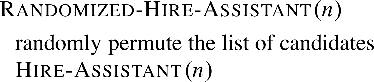
\includegraphics{Randomized-Hire-Assistant.pdf}

\vfill
\bi
\item
The randomization is now in the algorithm, not in the input distribution.
\item
Given a particular input, we can no longer say what its hiring cost will be. Each
time we run the algorithm, we can get a different hiring cost.
\item
In other words, each time we run the algorithm, the execution depends on the
random choices made.
\item
No particular input always elicits worst-case behavior.
\item
Bad behavior occurs only if we get ``unlucky'' numbers from the
randomnumber generator.
\ei

\end{frame}

\sect{Randomizing the hiring problem}

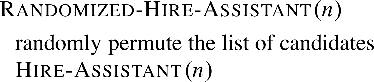
\includegraphics{Randomized-Hire-Assistant.pdf}

\vfill

\bi
\item
  The expected hiring cost is $O(c_h\lg n)$, regardless of input.
  \ei

\end{frame}

\sect{Randomly permuting an array}


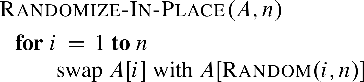
\includegraphics{Randomize-In-Place.pdf}
\vfill

\bi
\item {\bf Goal:}  Produce a uniform random permutation.

  (Each of the $n!$ permutations is equally likely.)


\item In iteration $i$, choose $A[i]$ randomly from $A[i..n]$.

\item
  Will never alter $A[i]$ after iteration $i$.
\item
  $O(1)$ per iteration, so $O(n)$.
  
\ei

\end{frame}

\sect{k-permutations}
\bi
\item
Given a set of $n$ elements, a {\bf k-permuation} is a sequence
containing $k$ of the $n$ elements.
\item
There are $n!/(n-k)!$ possible $k$-permutations.
\ei
\end{frame}


\sect{Algorithm computes a uniform random
  permutation}
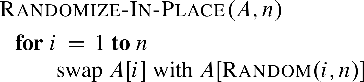
\includegraphics{Randomize-In-Place.pdf}
\vfill
\bi
\item {\bf Loop invariant:}
  Just prior to the $i$th iteration, for each possible
  $(i-1)$-permutation,  $A[1..i-1]$ contains this $(i-1)$-permutation
  with probability $(n-i+1)!/n!$.
  \pause
  \vfill
\item {\bf Initialization:}
  Just before iteration 1, $A[1..0]$ contains the 0-permutation with
  probability 1.

\ei
\end{frame}

\sect{Algorithm computes a uniform random
  permutation}
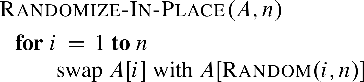
\includegraphics{Randomize-In-Place.pdf}
\bi
\item {\bf Loop invariant:}
  Just prior to the $i$th iteration, for each possible
  $(i-1)$-permutation,  $A[1..i-1]$ contains this $(i-1)$-permutation
  with probability $(n-i+1)!/n!$.
\item {\bf Maintenance:}
  \pause
\bi
\item
  Consider a $i$-permutation $\pi = (x_1,x_x,...x_i)$ .
\item
  It consists of $\pi' = (x_1,x_x,...x_{i-1})$ followed by $x_1$.
\item
  Let $E_1$ be the event that $\pi'$ is in $A[1..i-1]$.
\item
  Let $E_2$ be the event that $x_i$ is put into $A[i]$.
  \begin{align*}
    \pr{E_2 \cap E_1} &= \pr{E_2 | E_1} \pr{E_1}\\
    &= \frac{1}{n-i+1} \cdot \frac{(n-i+1)!}{n!} \\
    &= \frac{(n-i)!}{n!}
  \end{align*}
  
\ei
\ei
\end{frame}


\sect{Algorithm computes a uniform random
  permutation}
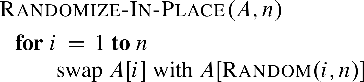
\includegraphics{Randomize-In-Place.pdf}
\vfill
\bi
\item {\bf Loop invariant:}
  Just prior to the $i$th iteration, for each possible
  $(i-1)$-permutation,  $A[1..i-1]$ contains this $(i-1)$-permutation
  with probability $(n-i+1)!/n!$.
\item {\bf Termination:}
  \pause
\item
  At termination, $i=n+1$, so $A[1..n]$ is a given $n$-permutation
  with probability
  \[
  \frac{(n-n)!}{n!} = \frac{1}{n!}
  \]
\ei
\end{frame}



\sect{The birthday paradox}
\bi
\item
How many people must be in a room before there is a 50\% chance of two
of them having the same birthday?
\pause
\item
  Assumptions:
\bi
\item
$\pr{b_i = r} = 1/n\mbox{ for }i=1..k\mbox{ and }r=1..n$
\item
$
    \pr{b_i=r \mbox{ and } b_j=r} =
    \pr{b_i=r}\pr{b_j=r} = 1/n^2
    $
    
    \ei
    \pause
\item Hence,
  the probability that two randomly selected people have the same birthday:
  \begin{align*}
    \pr{b_i = b_j}
    &=
    \sum_{i=1}^n \pr{b_i=r\mbox{ and } b_j=r}\\
    &=
    \sum_{i=1}^n (1/n^2)\\
    &= 1/n
  \end{align*}

\ei
\end{frame}

\sect{The birthday paradox}
\bi
\item
  The probability that two or more people have the same
  birthday, is 1 minus the probability that everybody's birthday
  is different.
\item Event that $k$ people have different birthdays:
  \begin{align*}
    B_k &= \bigcap_{i=1}^k A_i\\
    A_i &= \set{\mbox{events where $i$'s birthday $\neq$ $j$'s,
        for all $j < i$}}
\\\\
    B_k &= A_k \cap B_{k-1}\\
    \pr{B_k} &= \pr{B_{k-1}}\pr{A_k | B_{k-1}}\\
    \pr{B_1} &= \pr{A_1} = 1\\
    \pr{A_k | B_{k-1}} &= (n-(k-1))/n
  \end{align*}
\item What is the recurrence?
\ei

\end{frame}

\sect{The birthday paradox}
  \begin{align*}
    \pr{B_k}
    &= \pr{B_1}\pr{A_2 | B_{1}}\pr{A_3 | B_{2}}\cdots\pr{A_k | B_{k-1}}\\
    &= 1\cdot\left(\frac{n-1}{n}\right)
    \cdot\left(\frac{n-2}{n}\right)
    \cdots
    \left(\frac{n-k+1}{n}\right)\\
    &= 1\cdot\left(1-\frac{1}{n}\right)
    \cdot\left(1-\frac{2}{n}\right)
    \cdots
    \left(1-\frac{k-1}{n}\right)
  \end{align*}
  \begin{align*}
    \pr{B_k}
    &\leq e^{-1/n}e^{-2/n}\cdots e^{-(k-1)/n} & \mbox{since } 1 + x &\leq e^x\\
    &= e^{-k(k-1)/2n} \leq 1/2 
  \end{align*}
  when $ -k(k-1)/2n \leq \ln(1/2)$, or
  \[k\geq \frac{1+\sqrt{1+(8\ln 2)n} }{ 2}= \Theta(\sqrt{n})\]


\end{frame}

\sect{The birthday paradox}
  \begin{align*}
    \pr{B_k}
    &\leq 1/2 
  \end{align*}
  when 
  \[k\geq \frac{1+\sqrt{1+(8\ln 2)n} }{ 2}= \Theta(\sqrt{n})\]
  \vfill
  When $k=365$ we must have $k\geq 23$.
  \pause
  
  \vfill

  On Mars, a year is $669$ days long, so we need 31 Martians.
\end{frame}

\sect{The birthday paradox using indicator RVs}
\begin{align*}
  X_{ij}
  &=
  I\set{\mbox{person $i$ and $j$ have the same birthday}}\\
  E[X_{ij}] &= \pr{\mbox{person $i$ and $j$ have the same birthday}}\\
  &= 1/n
\end{align*}
Expected number of pairs of people with the same birthday:
\begin{align*}
  X &= \sum_{i=1}^{k-1}\sum_{j=i+1}^{k} X_{ij}\\
  E[X] &= E\left[\sum_{i=1}^{k-1}\sum_{j=i+1}^{k} X_{ij}\right]\\
   &= \sum_{i=1}^{k-1}\sum_{j=i+1}^{k} E[X_{ij}]\\  
  &= \binom{k}{2}\frac{1}{n} = \frac{k(k-1)}{2n}
\end{align*}

\end{frame}


\sect{The birthday paradox using indicator RVs}
\bi
\item
  Expected number of pairs of people with the same birthday:
  \begin{align*}
    E[X]  &= \frac{k(k-1)}{2n}\\
    E[X] \geq 1 &\Longleftrightarrow k(k-1) \geq 2n
  \end{align*}
\item
  Thus, if we have at least $\sqrt{2n}+1$ people in the room,
  we can expect at least two have the same birthday.
\item
  On earth, 28 people will make the expected value 1.0356.
\item
  On Mars, 38 Martians are needed.
  \pause
\ei  
\end{frame}

\sect{Difference between the analyses}
\bi
\item First analysis determined the number necessary for the
  probability of at least two people with the same birthday
  to exceed 1/2.
\item
  Second analysis determined the number necessary for the expected
  number of pairs of matching birthdays to be at least 1.
\item
  The exact numbers differ, but both are $\Theta(\sqrt{n})$.
\ei

\end{frame}
\end{document}
